\documentclass[9pt,fleqn]{article}
\usepackage[margin=0.5in]{geometry}
\usepackage{multicol}
\usepackage{lipsum}% dummy text
\usepackage[fleqn]{amsmath}
\usepackage[compact]{titlesec}
\usepackage{graphicx}

\setlength{\mathindent}{0pt}
\setlength{\columnseprule}{0pt}
\setlength{\parskip}{0pt}
\setlength{\parindent}{0pt}
\setlength\abovedisplayskip{0pt}
\setlength\belowdisplayskip{0pt}
\setlength{\jot}{0pt}
\linespread{0.9}

\allowdisplaybreaks

\begin{document}
\begin{multicols}{3}

    \section*{General}
    \textbf{Demorgans Law}
    \begin{flalign*}
        \neg[p\wedge q]\equiv\neg p\vee\neg q,\\
        \neg[p\vee q]\equiv\neg p\wedge\neg q.
    \end{flalign*}
    \textbf{Rise/Fall time}
    \begin{flalign*}
        t_{r} = R_{p}C ,
        t_{f} = R_{n}C \\
        R_{n} \propto {L_{n} \over W_{n}\mu_{0_{n}}},
        R_{p} \propto {L_{p} \over W_{p}\mu_{0_{p}}}
    \end{flalign*}
    \textbf{Elmore's delay}
    \begin{flalign*}
        &\tau_{Di} = \sum_{k=1}^{N} C_{k}*R_{ik} \\
        &Estimated Delay = \tau_{p} = 0.69*\tau_{Di} \\
        &Total Expected Energy = C_{L}*f*{{V_{dd}}^2}
    \end{flalign*}
    \textbf{Power Probability}
    \begin{flalign*}
        P_{n\_nand}(0) &= P_{A}(1)P_{B}(1) \\
        P_{p\_nand}(1) &= 1-P_{A}(1)P_{B}(1) \\
        P_{n\_nor}(0)  &= 1-P_{A}(0)P_{B}(0) \\
        P_{p\_nor}(1)  &= P_{A}(0)P_{B}(0)
    \end{flalign*}
    \textbf{Fan out}
    \begin{flalign*}
        f = \sqrt[N]{{C_{L} \over C_{1}}}
    \end{flalign*}
    \textbf{Min Path Delay}
    \begin{flalign*}
        t_{p} = N*t_{po}*(1 + f)
    \end{flalign*}

    \subsection*{Gates}
    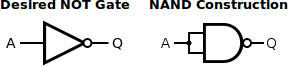
\includegraphics[width=\linewidth]{not.png}
    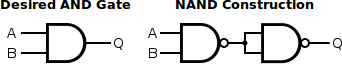
\includegraphics[width=\linewidth]{and.png}
    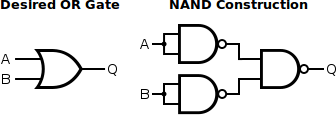
\includegraphics[width=\linewidth]{or.png}
    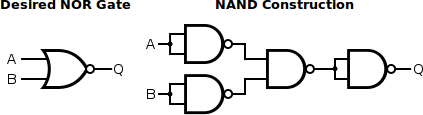
\includegraphics[width=\linewidth]{nor.png}
    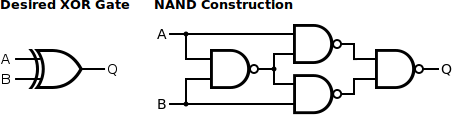
\includegraphics[width=\linewidth]{xor.png}
    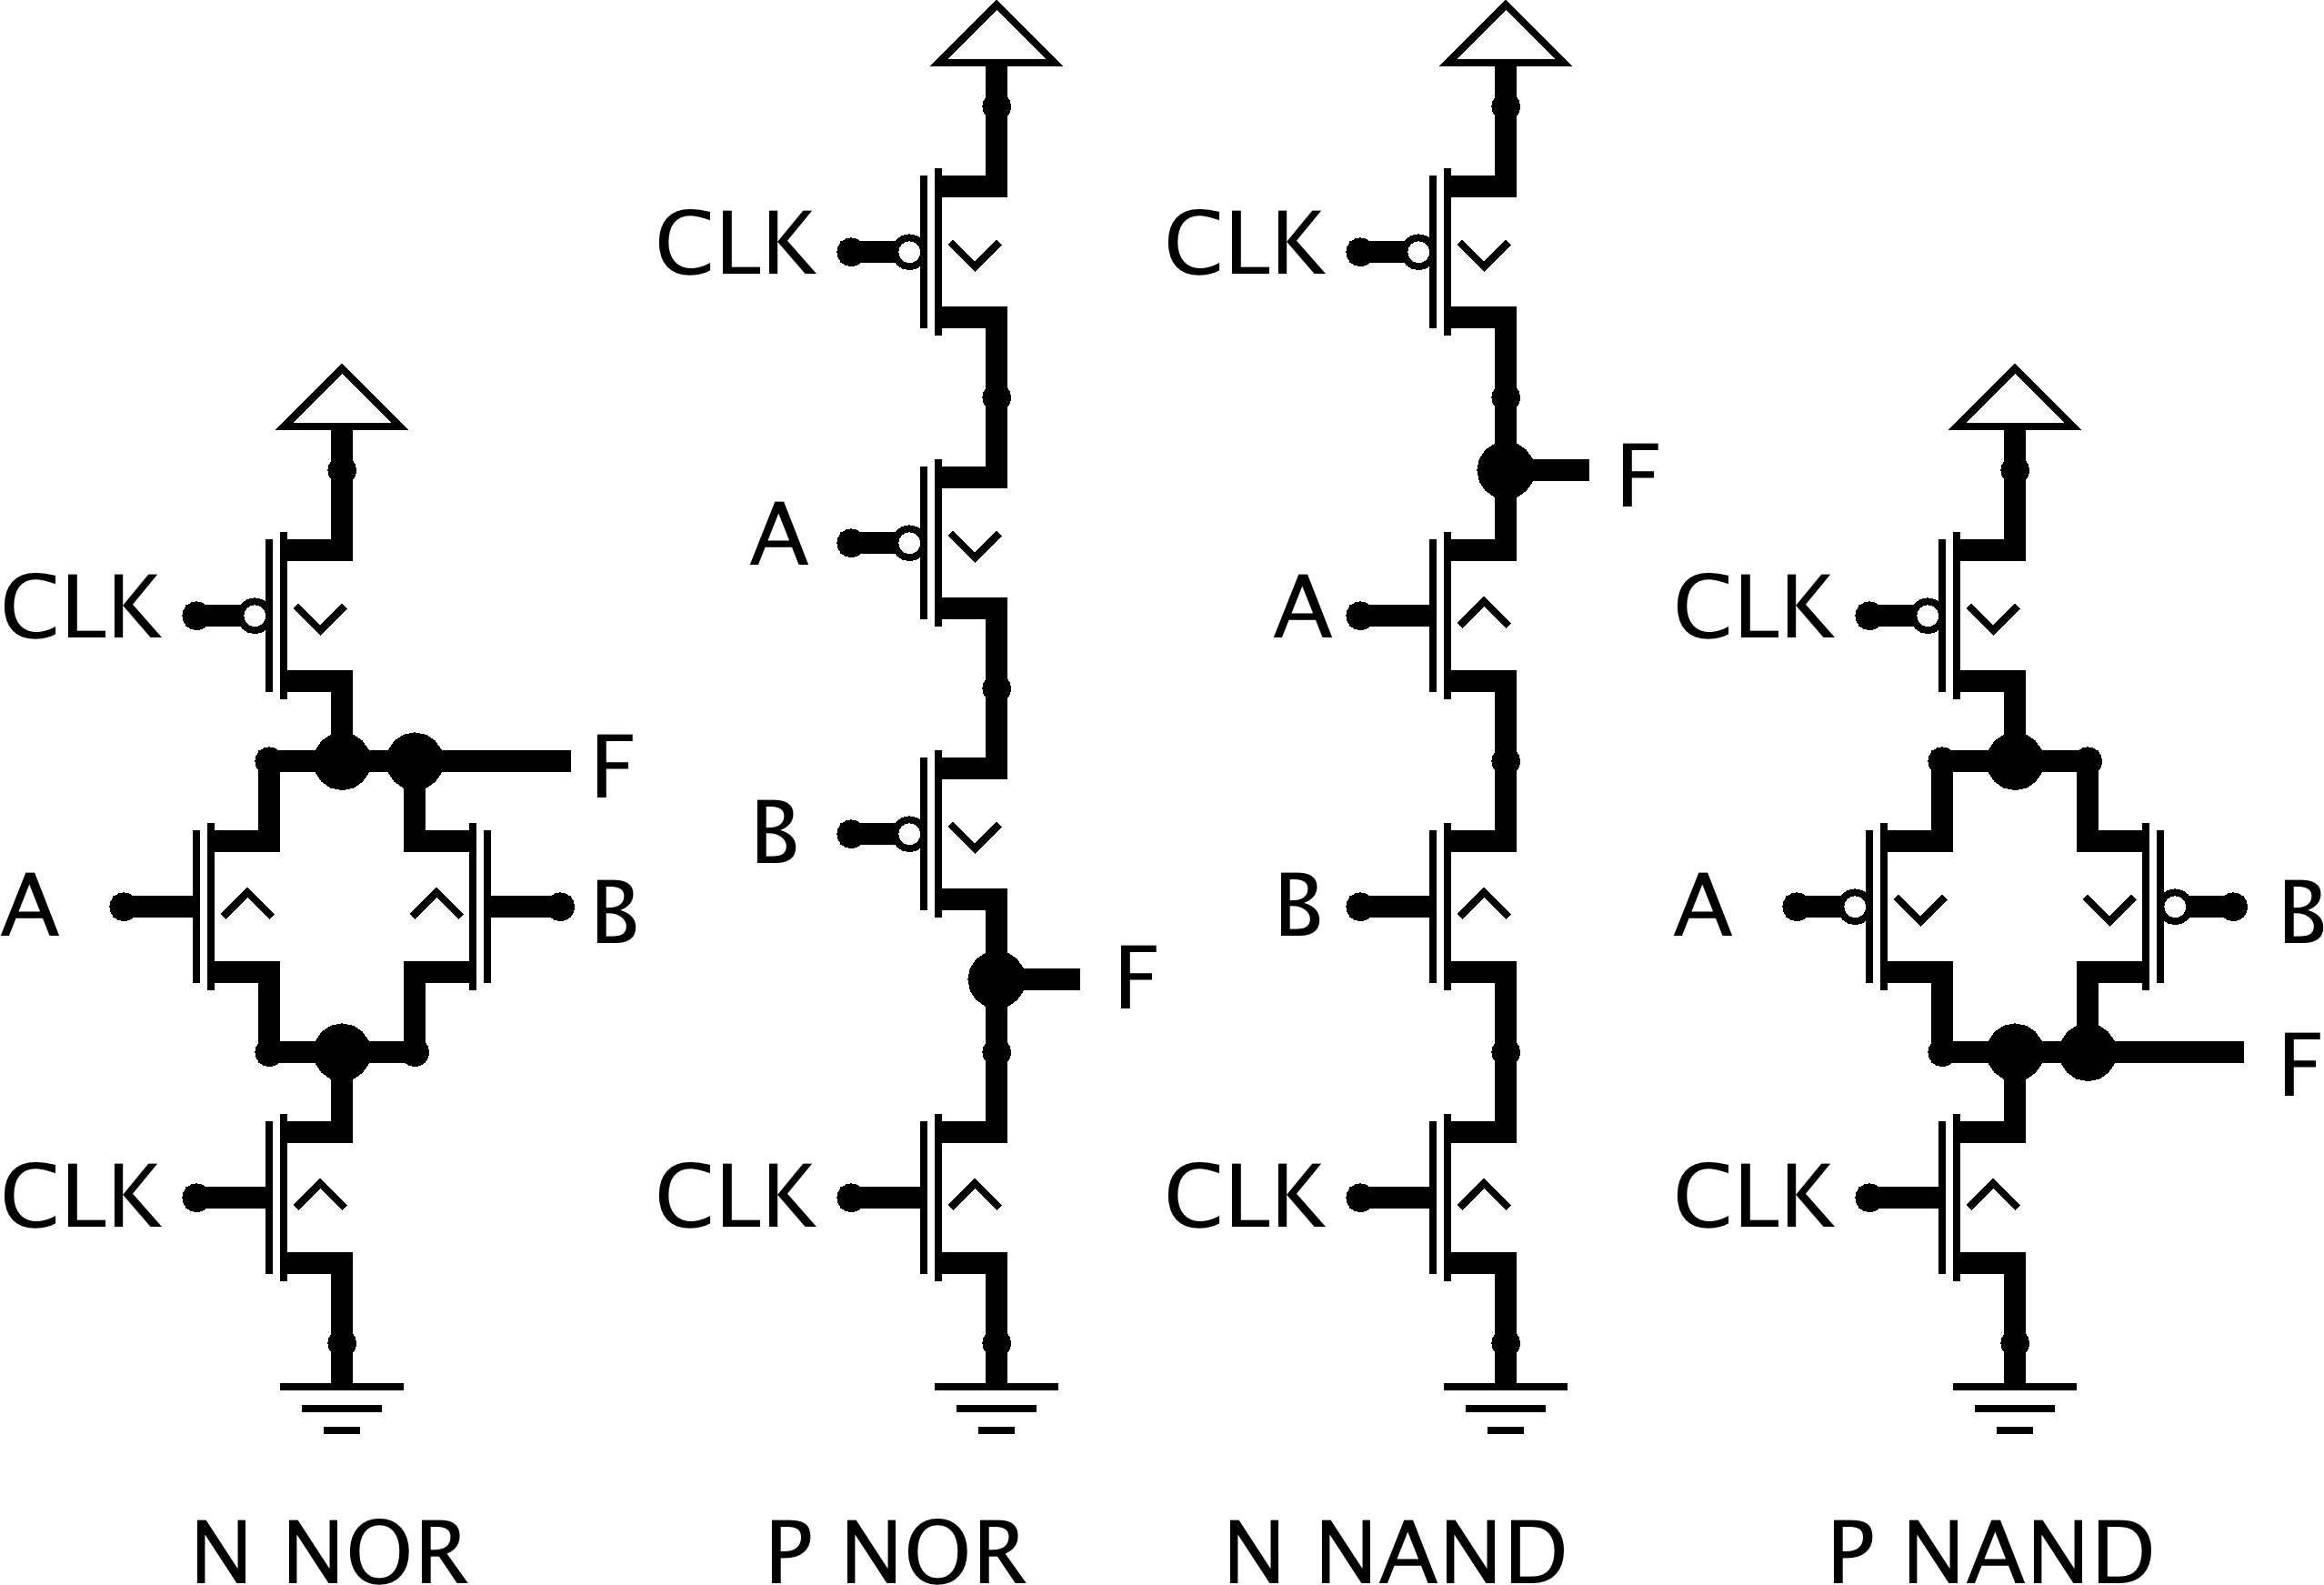
\includegraphics[width=\linewidth]{dynamic_gates.png}

    \subsection*{Definitions}
    \textbf{Inertial Delay -} time it takes for signal to change value \\
    \textbf{Transport Delay -} time it takes for signal to travel down wire \\
    \textbf{Delta Cycle -} is used to order events in VHDL simulation and
    refers to a zero-physical time. The kernel takes an additional cycle (of
    delta advancement) to update the evaluated 'future value' into the 'current
    value' registers, during which the clock doesn't advance. \\
    \textbf{Channel Length Modulation -} shorting of the length of the inverted
    channel region with increase in drain bias for large drain biases \\
    \textbf{Velocity Saturation -} carrier velocity reaches maximum value in
    presence of electric field. \\
    \textbf{Latch up -} a short circuit in which a low impedance path is
    created resulting in a parasitic subcircuit that disrupts proper function.\\
    \textbf{Velocity Saturation -} when a strong enough electric field is
    applied, the carrier velocity in the semiconductor reaches a maximum value.
    As the applied electric field increases from that point, the carrier
    velocity no longer increases because the carriers lose energy through
    increased levels of interaction with the lattice, by emitting phonons and
    even photons as soon as the carrier energy is large enough to do so.\\
    \textbf{Hot Carrier -} Either holes or electrons  that have gained very
    high kinetic energy after being accelerated by a strong electric field in
    areas of high field intensities within a semiconductor .  Because of high
    kinetic energy they can get injected and trapped in areas of the device
    where they shouldn't be.\\
    \textbf{Scan Chain -} is a technique used for testing digital circuits. The
    flip flops are all connected together as a shift register into a single (or
    multiple) scan chains. It increases observability and controllability in
    the design and also helps to reduce the size of the test-set vector. \\
    \textbf{Process gain factor -}
        \begin{flalign*}
            K = \mu \epsilon_{iO_{2}} \over t_{ox}
        \end{flalign*}
    \textbf{Intrinsic Capacitance - } refers to the internal capacitance of a
    static gate generated dude to diffusion layers, metal contacts, poly-wires.
    The parasitic capacitance is proportional to the dimensions of the gate
    (i.e. W and L of transistor).  As we increase the size of the gate, the
    intrinsic capacitance increases, in turn increasing the delay of the gate.
    We aim to reduce intrinsic capacitances, but it can never be made '0'.\\
    \textbf{TSPCR -} True Single Phase Clock Register performs the flip-flop
    operation with little power and at high speeds. Stores output using
    capacitance. Will typically not work at static or low clock speeds: given
    enough time, leakage paths may discharge the parasitic capacitance enough
    to cause the flip-flop to enter invalid states.\\
    \textbf{Master Slave FF -} Is edge trigged. Two gated D latches in series
    and and inverting the enable input to one of them.

\end{multicols}
\end{document}
